\documentclass[a4paper,11pt]{article}

\usepackage[utf8]{inputenc}
\usepackage[T1]{fontenc}
\usepackage{mathptmx}

\usepackage[a4paper,text={160mm,220mm},centering]{geometry}

\usepackage{hyperref}
\usepackage{listings}
\usepackage{graphicx}
\usepackage[table]{xcolor}

\lstset{basicstyle={\ttfamily}}

\usepackage{todonotes}

\begin{document}

\thispagestyle{empty}

\unitlength=1mm
\begin{picture}(140,30)
\put(-10,30){\includegraphics[height=12mm]{../images/TIS-logo.png}}
\put(-10,11){
\includegraphics[height=22mm]{../images/adacore.png}}
\put(-6,0){
\includegraphics[height=12mm]{../images/logo_ocamlpro.png}}
\put(125,30){
\includegraphics[height=10mm]{../images/Universite_Paris_Saclay_logo.png}}
\put(127,12){
\includegraphics[height=16mm]{../images/cnrs.png}}
\put(123,0){
\includegraphics[height=12mm]{../images/logo-inria-reduced.png}}
\end{picture}

\vfill

\begin{center}

{  \Huge\bfseries
  Projet Décysif --- Livrable 2.1 }

\bigskip

{  \LARGE\bfseries
Constitution d’une base de fichiers d’entrée
représentatifs des difficultés rencontrées pour la
preuve automatique.}


\vfill

\large Juillet 2024

\vfill

\large Yannick Moy (AdaCore), Guillaume Cluzel (TrustInSoft), Matteo
Manighetti (Inria \& Université Paris-Saclay), Claude Marché (Inria \& Université Paris-Saclay)


\end{center}

\vfill

\noindent\begin{picture}(140,30)
\put(0,0){
\includegraphics[width=0.3\textwidth]{../images/Logo_Bpifrance.png}}
\put(70,0){
\includegraphics[width=0.3\textwidth]{../images/LOGO_RIDF_2019_COULEUR.png}}
\put(145,0){
\includegraphics[width=0.1\textwidth]{../images/Logo-France-2030-rouge-bleu.png}}
\end{picture}

\noindent Le projet Décysif est financé par la Région Île-de-France et par le Gouvernement
Français dans le cadre du Plan France 2030

\clearpage


Ce livrable est constituée d'une base de tests qui se trouve dans le dépot
\href{https://github.com/Decysif/benchmarks}{'benchmarks'} du projet Décysif.

Objectifs du livrable :

\begin{itemize}
\item Repérer les faiblesses du prouveur Alt-Ergo
\item Repérer les problèmes de traduction (ou repérer des problèmes au niveau de l'écriture des théories, par exemple le modèle mémoire de J3) pour tous les prouveurs cvc5, CVC4, Z3, Alt-Ergo.
\end{itemize}

% Une section par répertoire d'exemples avec une description du contenu
% et de la méthodologie des statisques adoptée. Et le résultat de ces statisques
% au démarrage du projet.

% Mettre les statistiques qu'on a quand elles existent.

\section{Exemples issus de Why3}

\subsection{Jeu d'exemples de programmes écrits en WhyML}

Le sous-répertoire \url{why3_examples} contient le jeu d'exemples
extrait du bench complet de Why3, formé de code source dans le langage
WhyML. La documentation de référence est dans le fichier \url{README.md} de ce répertoire.
Pour installer et configurer ce jeu de tests, la commande
\begin{lstlisting}
> ./import_suite.sh
\end{lstlisting}
doit être exécutée au préalable. Ceci récupère une version de
référence de Why3 (1er mars 2024) et compile les commandes nécessaires. Ensuite la commande
\begin{lstlisting}
> ./run_bench.sh
\end{lstlisting}
pour être lancée pour executer les tests proprement dit. Les prouveurs
utilisés pour ces tests sont indiqués dans le fichier
\url{run_bench.sh} lui-même.

Une exécution de référence de ces tests a été lancée le 15 avril 2024
sur le serveur de calcul «~moloch~» de l'équipe Inria Toccata. Ce
serveur dispose de 16 c{\oe}urs «~Intel(R) Xeon(R) CPU E5-2450 v2 @
2.50GHz~» et de 64 Go de memoire centrale. Pour ces tests, 8 c{\oe}urs
ont été utilisés. Sur chaque fichier source, on demande à Why3 de
générer l'obligation de preuve de chaque fonction, de découper la
formule générée en plusieurs sous-formules, puis on appelle un jeu de
prouveur sur chacune des sous-formules. Un temps limite de 5 secondes est donné à chaque exécution de prouveurs. Pour l'exécution de référence,
les prouveurs Alt-Ergo 2.5.2, CVC4 1.8, cvc5 1.0.5 et Z3 4.12.2 ont
été utilisés. Les résultats sont enregistrés dans des fichiers de
session de preuve de Why3, pouvant donner lieu à diverses
statistiques. Voici des statistiques globales pour l'exécution de
référence, le nombre total d'obligation de preuve est de 41389:
\begin{center}
  \rowcolors{2}{gray!25}{white}
  \begin{tabular}{|l|r|r|r|r|r|}
    \hline
  \rowcolor{gray!50} Prouveur
  & \multicolumn{1}{p{0.13\textwidth}|}{nombre de buts}
  & \multicolumn{1}{p{0.13\textwidth}|}{nombre de buts prouvés}
  & \multicolumn{1}{p{0.13\textwidth}|}{temps minimal}
  & \multicolumn{1}{p{0.13\textwidth}|}{temps maximal}
  & \multicolumn{1}{p{0.13\textwidth}|}{temps moyen}
  \\
  Alt-Ergo 2.5.2                & 41389 & 32170 &  0.00  & 4.98 &  0.12 \\
  CVC4 1.8                      & 41389 & 33650 &  0.01  & 4.81 &  0.17 \\
  cvc5 1.0.5                    & 41389 & 32904 &  0.01  & 4.92 &  0.17 \\
    Z3 4.12.2                     & 41389 & 30713 &  0.01  & 4.96 &  0.07 \\
    \hline
\end{tabular}
\end{center}

\begin{figure}
  \centering
  \hspace*{-0.1\textwidth}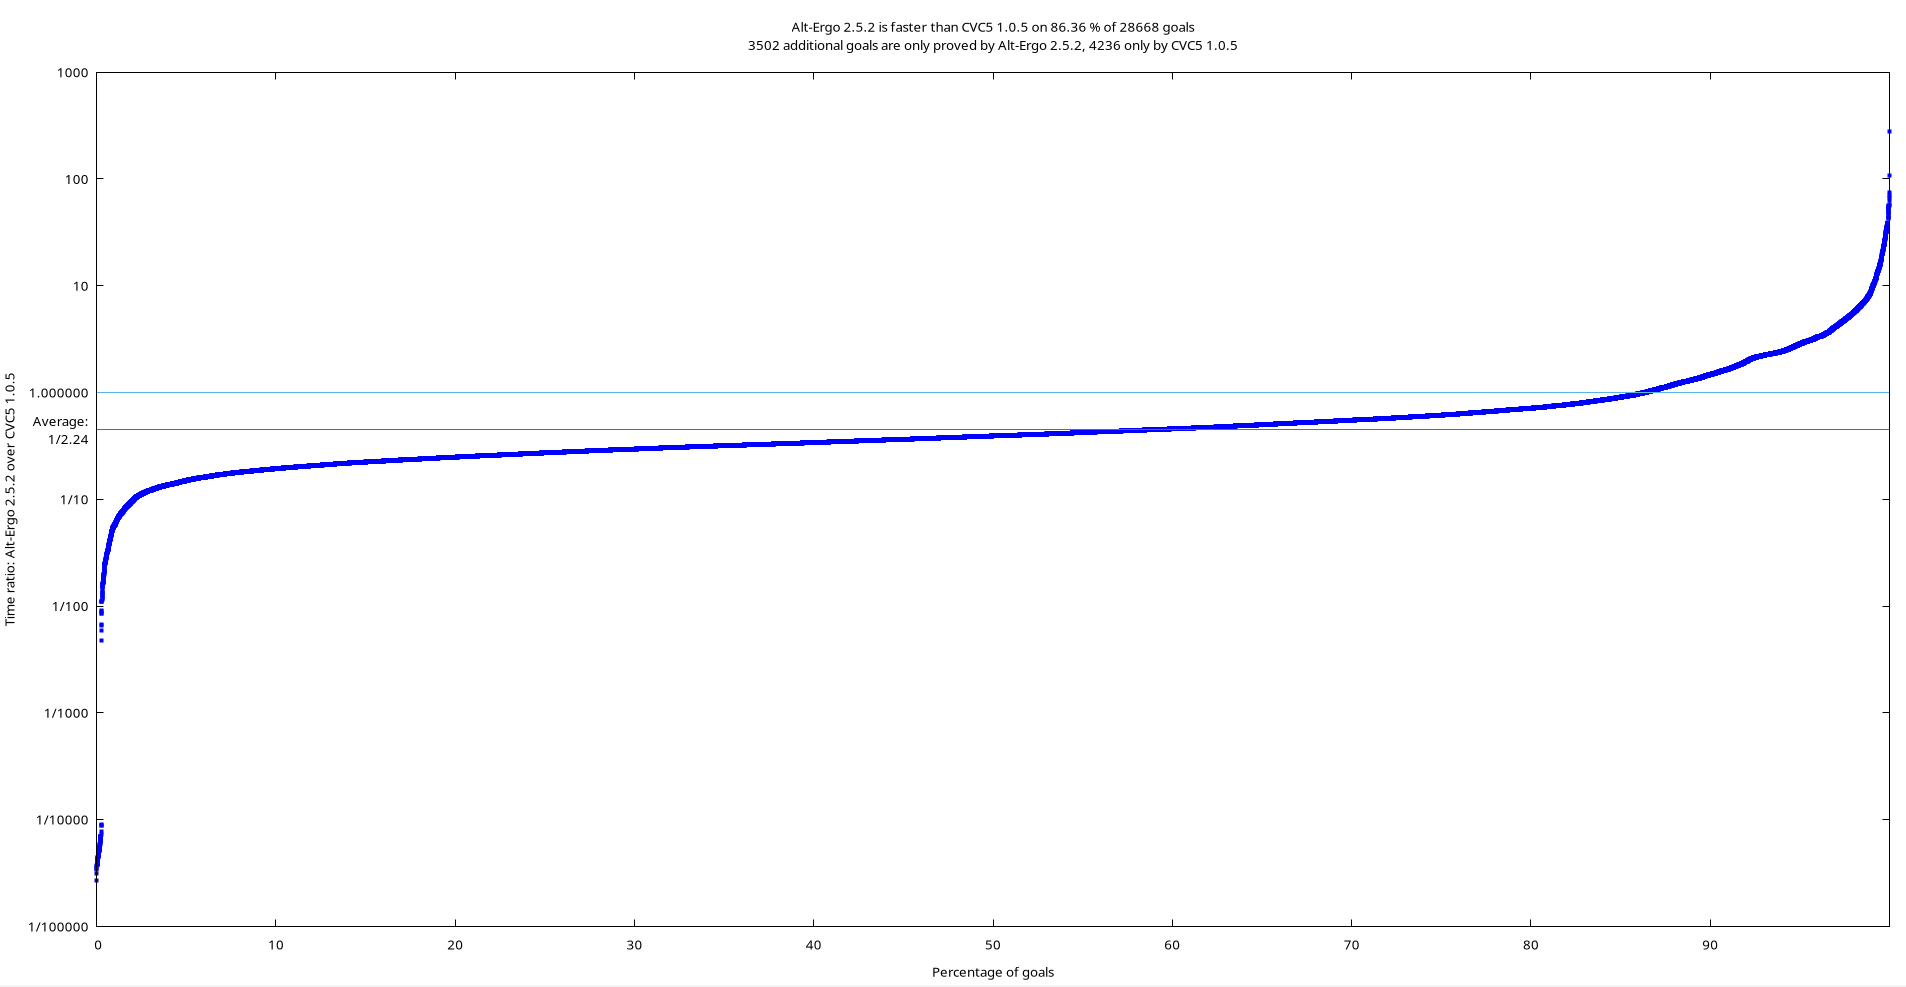
\includegraphics[width=1.2\textwidth]{AE-vs-CVC5.png}
  \caption{Comparaison d'Alt-Ergo et cvc5. Globalement, cvc5 prouve
    plus de buts qu'Alt-Ergo, mais Alt-Ergo est plus rapide. On
    indique aussi que 3502 buts sont prouvés par Alt-Ergo mais pas par
    cvc5, alors que 4236 sont prouvés par cvc5 mais pas par Alt-Ergo.}
  \label{fig:AEvsCVC5}
  \hrulefill
\end{figure}

Des statistiques plus fines peuvent être calculées à la demande sur
les fichiers de sessions. Par exemple, la figure~\ref{fig:AEvsCVC5}
une représentation graphique qui compare les performances de Alt-Ergo
et de cvc5 sur le jeu de test.

En fin de projet, une exécution similaire des outils améliorés seront
rejoués sur les même exemples, et on évaluera les améliorations
apportées en terme de pourcentage de preuve automatique réussies.

\subsection{Exemples écrits spécifiquement pour le projet Décysif}

Le répertoire \url{why3_handcrafted} contient un nombre réduits
d'exemples, qui ont été écrits en WhyML pour spécifiquement tester les
capacités de preuve automatiques des prouveurs. Ces exemples sont
sélectionnés comme représentatifs des difficultés que l'on cherche à
résoudre. L'idéal sera qu'en fin de projet, tous les exemples en
question soient prouvés automatiquement.

Il n'y a pas de statistiques initiales pour ces exemples, car au début
du projet ce sont tous spécifiquement des exemples qui ne sont pas
prouvés.

\section{Exemples issus de J3}

\subsection{Jeu d'exemples de programmes écrits en C et extraits en WhyML}

Le sous-répertoire \url{j3_example} contient le jeu d'exemples extrait du bench
d'exemples de la distribution de SPARK, formé de code source dans le langage C.
La documentation de référence est dans le fichier \url{README.md} de ce
répertoire.

La création de ce jeu de tests se fait via la lancement d'un script
\verb/generate-sexp.sh/.
Ce script nécessite d'avoir le binaire \verb/tis-analyzer/ qui sera lancé
pour générer les fichiers sexp sur tous les exemples présents dans ce
répertoire.

Un deuxième script \verb/run.sh/ permet de lancer Why3 sur tous les fichiers
sexp préalablement générés. Why3 tente ensuite de faire prouver les obligations
de preuve généré par les prouveurs Alt-Ergo 2.5.2, CVC4 1.8, cvc5 1.0.8 et
Z3 4.8.17. Une exécution de référence de ces tests a été lancé le 6 juin 2024
sur une machine disposant de 12 c{\oe}urs «~11th Gen Intel(R) Core(TM) i7-11800H @ 2.30GHz~» et disposant de 16~Go de RAM.
Les résultats sont enregistrés dans de fichier de session de preuve et peuvent
donner lieu à plusieurs statistiques.
Voici des statistiques globales pour l'exécution de
référence, le nombre total d'obligation de preuve est de 9534:

\begin{center}
  \rowcolors{2}{gray!25}{white}
  \begin{tabular}{|l|r|r|r|r|r|}
    \hline
  \rowcolor{gray!50} Prouveur
  & \multicolumn{1}{p{0.13\textwidth}|}{nombre de buts}
  & \multicolumn{1}{p{0.13\textwidth}|}{nombre de buts prouvés}
  & \multicolumn{1}{p{0.13\textwidth}|}{temps minimal}
  & \multicolumn{1}{p{0.13\textwidth}|}{temps maximal}
  & \multicolumn{1}{p{0.13\textwidth}|}{temps moyen}
  \\
  Alt-Ergo 2.5.2                &  9534 & 5321 & 0.05 & 4.98 & 0.18 \\
  CVC4 1.8                      &  9534 & 7533 & 0.04 & 4.77 & 0.28 \\
  cvc5 1.0.8                    &  9534 & 7500 & 0.03 & 4.96 & 0.31 \\
  Z3 4.8.17                     &  9534 & 6948 & 0.02 & 4.93 & 0.61 \\
    \hline
\end{tabular}
\end{center}

Des statistiques plus fines peuvent être extraites pour comparer deux à deux
les prouveurs utilisés pour la preuve et affichant le résultat sous une forme
similaire à celle présentée dans la section précédente. Ces résultats peuvent
être trouvés dans le sous-dossier \url{results/2024-06-06}.

\subsection*{Examples écrits spécifiquement pour le projet}

Le dossier \url{j3_handcrafted} contient des examples de programmes C
relativement basiques qui mettent en échec les différents prouveurs CVC4, cvc5,
Z3 et Alt-Ergo dans leurs versions mentionnées précédemment.
Ces exemples ont été sélectionnés car représentatifs des problèmes que l'on
cherche à résoudre, et ils semblent suffisamment simples pour que l'ont puisse
s'attendre à qu'ils soient prouvés automatiquement.

\section{Exemples issus de SPARK}

\subsection{Jeu d'exemples de programmes écrits en SPARK et extraits vers WhyML}

Le sous-répertoire \url{spark_examples} contient le jeu d'exemples extrait du
bench d'exemples de la distribution de SPARK, formé de code source dans le
langage SPARK. La documentation de référence est dans le fichier
\url{README.md} de ce répertoire.

Le code archivé correspond au code Why3 extrait du code SPARK par l'exécution
de gnatprove. Pour installer et configurer ce jeu de tests, les commandes
\begin{lstlisting}
> unzip spark_sexp.zip
> export PATH=$PWD/../why3_examples/why3-88dc033/bin:$PATH
> ./build_environment.sh
> make
\end{lstlisting}
doivent être exécutées au préalable. Cela suppose que le setup dans \url{why3_examples}
a été effectué au préalable afin de récupèrer une version de
référence de Why3 (1er mars 2024) et de compiler les commandes nécessaires. Ensuite la commande
\begin{lstlisting}
> ./run_bench.sh
\end{lstlisting}
doit être lancée pour exécuter les tests proprement dit. Les prouveurs
utilisés pour ces tests sont indiqués dans le fichier
\url{run_bench.sh} lui-même.

Une exécution de référence de ces tests a été lancée le 11 juin 2024
sur le serveur de calcul «~moloch~» de l'équipe Inria Toccata. Ce
serveur dispose de 16 c{\oe}urs «~Intel(R) Xeon(R) CPU E5-2450 v2 @
2.50GHz~» et de 64 Go de memoire centrale. Pour ces tests, 8 c{\oe}urs
ont été utilisés. Sur chaque fichier source, on demande à Why3 de
générer l'obligation de preuve de chaque fonction, de découper la
formule générée en plusieurs sous-formules, puis on appelle un jeu de
prouveur sur chacune des sous-formules. Un temps limite de 5 secondes est donné à chaque exécution de prouveurs. Pour l'exécution de référence,
les prouveurs Alt-Ergo 2.4.0, cvc5 1.0.5 et Z3 4.12.4 ont
été utilisés, avec les drivers propres à GNATprove.
Les résultats sont enregistrés dans des fichiers de
session de preuve de Why3, pouvant donner lieu à diverses
statistiques. Voici des statistiques globales pour l'exécution de
référence, le nombre total d'obligation de preuve est de 135036:
\begin{center}
  \rowcolors{2}{gray!25}{white}
  \begin{tabular}{|l|r|r|r|r|r|}
    \hline
  \rowcolor{gray!50} Prouveur
  & \multicolumn{1}{p{0.13\textwidth}|}{nombre de buts}
  & \multicolumn{1}{p{0.13\textwidth}|}{nombre de buts prouvés}
  & \multicolumn{1}{p{0.13\textwidth}|}{temps minimal}
  & \multicolumn{1}{p{0.13\textwidth}|}{temps maximal}
  & \multicolumn{1}{p{0.13\textwidth}|}{temps moyen}
  \\
  Alt-Ergo 2.4.0                & 135036 &  98822 &  0.00  & 4.96 &  0.09 \\
  cvc5 1.0.5                    & 135036 & 100560 &  0.01  & 4.98 &  0.11 \\
  Z3 4.12.4                     & 135036 & 101915 &  0.00  & 4.89 &  0.04 \\
\hline
\end{tabular}
\end{center}

\subsection{Jeu d'exemples de VC écrites en SMT-LIB2}

Le sous-répertoire \url{spark_handcrafted} contient le jeu d'exemples de VC
écrites directement au format SMT-LIB2 à partir de VC provenant de la suite de
tests SPARK, représentatives des difficultés observées pour prouver des
propriétés arithmétiques. La documentation de référence est dans le fichier
\url{README.md} de ce répertoire.

Les scripts nécessaires pour comparer les résultats de différents prouveurs sur
ces VC sont disponibles dans le sous-répertoire \url{spark_scripts}. Le détail
des commandes est indiqué dans le fichier \url{README.md}. Les résultats sont
enregistrés dans le sous-répertoire \url{results}.  Pour l'exécution de
référence, les prouveurs Alt-Ergo 2.4.0, cvc5 1.0.5 et Z3 4.12.4 et Colibri
2020.9 ont été utilisés.

\begin{center}
  \rowcolors{2}{gray!25}{white}
  \begin{tabular}{|l|r|r|r|}
    \hline
  \rowcolor{gray!50} Prouveur
  & \multicolumn{1}{p{0.13\textwidth}|}{arithmétique entière (51 VC)}
  & \multicolumn{1}{p{0.13\textwidth}|}{arithmétique de bit-vecteurs (20 VC)}
  & \multicolumn{1}{p{0.13\textwidth}|}{arithmétique mixte entière et bit-vecteurs (8 VC)}
  \\
  Alt-Ergo 2.4.0                &  8 &  0 & 0  \\
  cvc5 1.0.5                    & 38 &  1 & 0 \\
  Z3 4.12.4                     & 43 &  1 & 3 \\
    Colibri 2020.9                & 23 & 11 & 1 \\
    \hline
\end{tabular}
\end{center}

\section{Exemples issus de Creusot}

Le répertoire \url{creusot_examples} contient un jeu de tests issus de
l'outil Creusot~\cite{denis22icfem}.

Ces exemples se présentent sous la forme de fichiers mlcfg, un format d'entrée supporté par Why3.

Les fichiers mlcfg intégrés ont été générés avec la version 0.1 de
Creusot.

Ce jeu est constitué d'une sélection d'exemples issus du
sous-répertoire \url{tests/should_succeed}. Cette sélection ignore
simplement les petits tests unitaires visant à tester des features
individuelles de Creusot.

Ce jeu de tests sera amené à etre complété à l'avenir (cf section de conclusion).

Une exécution de référence de ces tests a été lancée le 3 juillet 2024
sur le serveur de calcul «~moloch~» de l'équipe Inria Toccata. Ce
serveur dispose de 16 c{\oe}urs «~Intel(R) Xeon(R) CPU E5-2450 v2 @
2.50GHz~» et de 64 Go de memoire centrale. Pour ces tests, 8 c{\oe}urs
ont été utilisés. Sur chaque fichier source, on demande à Why3 de
générer l'obligation de preuve de chaque fonction, de découper la
formule générée en plusieurs sous-formules, puis on appelle un jeu de
prouveur sur chacune des sous-formules. Un temps limite de 5 secondes est donné à chaque exécution de prouveurs. Pour l'exécution de référence,
les prouveurs Alt-Ergo 2.5.4, CVC4 1.8, cvc5 1.0.5 et Z3 4.12.2 ont
été utilisés. Les résultats sont enregistrés dans des fichiers de
session de preuve de Why3, pouvant donner lieu à diverses
statistiques. Voici des statistiques globales pour l'exécution de
référence, le nombre total d'obligation de preuve est de 4706:
\begin{center}
  \rowcolors{2}{gray!25}{white}
  \begin{tabular}{|l|r|r|r|r|r|}
    \hline
  \rowcolor{gray!50} Prouveur
  & \multicolumn{1}{p{0.13\textwidth}|}{nombre de buts}
  & \multicolumn{1}{p{0.13\textwidth}|}{nombre de buts prouvés}
  & \multicolumn{1}{p{0.13\textwidth}|}{temps minimal}
  & \multicolumn{1}{p{0.13\textwidth}|}{temps maximal}
  & \multicolumn{1}{p{0.13\textwidth}|}{temps moyen}
  \\
  Alt-Ergo 2.5.4                &  4706  & 4333   & 0.00  & 4.87  & 0.06 \\
  CVC4 1.8                      &  4706  & 4219   & 0.01  & 4.52  & 0.09 \\
  cvc5 1.0.5                    &  4706  & 4392   & 0.01  & 4.88  & 0.11 \\
  Z3 4.12.2                     &  4706  & 4319   & 0.00  & 4.50  & 0.07 \\
  \hline
\end{tabular}
\end{center}



\section{Travail futur}

Les statistiques présentées mettent en avant les nombres totaux de VC prouvées
par chaque prouveur. D'autres statistiques seront utiles, concernant le nombre
de VC prouvées par un seul ou aucun prouveur. Nous les incluerons dans le futur.

Les résultats actuels vont nous permettre de travailler avec les équipes de
développement des prouveurs automatiques, en particulier Alt-Ergo, pour
améliorer leurs résultats sur les différentes suites de test. Nous suivrons les
effets de ces améliorations sur les tests rassemblés pour ce rapport initial.

Nous désirons également mesurer les résultats d'autres prouveurs sur ces suites
de tests, comme le successeur Colibri2 de Colibri, et les prouveurs dReal et
Gappa spécialisés pour les problèmes d'arithmétique en virgule flottante.

Dans le cadre de J3, nous aimerions égalemnt constituer une suite de tests
constitués de quelques exemples de code C++ possédant leur propres spécificités.

Dans le futur, nous penson également compléter le jeu de test de
Creusot par des exemples complexes, on pense à CreuSAT~\cite{skotam22creusat}
(\url{https://github.com/sarsko/creusat}) et cdsat
(\url{https://github.com/xldenis/cdsat}). Par ailleurs, il se trouvent
que dans son fonctionnement, Creusot fait une usage particulier de la
théorie des séquences, qui semble être une théorie diffficle pour les
prouveurs. On pourra donc être amené à isoler dans notre jeu de tests
les exemples qui échouent à cause des séquences, afin de fournir un
jeu de test réduit pour ce cas précis.

\clearpage

\bibliographystyle{plainurl}
\bibliography{generated,main}
%\bibliography{abbrevs,demons,demons2,demons3,team,crossrefs}

\end{document}
